\documentclass[conference]{IEEEtran}
\IEEEoverridecommandlockouts

\usepackage{amsmath,amssymb,amsfonts}
\usepackage{graphicx}
\usepackage{textcomp}
\usepackage{booktabs}
\usepackage{tabularx}
\usepackage{url}

% REVISION NOTES (for authors --- remove before final submission):
% R1. Literature survey orphan citations replaced with \cite{} commands to bib entries.
% R2. Keywords: removed \textbf{}, reduced to 6 terms per IEEEtran convention.
% R3. Confusion matrix: TN+FP row total corrected to 11,183 (arith. match).
%     Total test count corrected to 17,026; normal beats to 11,183 per split manifest.
%     NEEDS AUTHOR VERIFICATION if different from frozen saved predictions.
% R4. "Operational" replaced with "evaluated" or "benchmark" throughout.
% R5. VitalDB test cohort 708,755: flagged as full dataset --- NEEDS AUTHOR VERIFICATION.
% R6. sub-50ms latency claim qualified with "on the development test server."
% R7. Emergency advisory numbers (112, 108) moved from Results to System Design.
% R8. LBM equations numbered.
% R9. Long parenthetical in Introduction split into two sentences.
% R10. Abstract condensed to ~175 words.
% R11. \cite{} commands embedded in dataset, method, and formula descriptions.
% R12. Holliday-Segar pediatric origin noted; GDT context added.
% R13. FPR alarm-fatigue implication added to Results and Limitations.
% R14. Calibration vs. discrimination note added after Brier scores.

\begin{document}

\title{ANESTHESIA DOSE CALCULATION AND SAFETY SUPPORT SYSTEM}

\author{
\IEEEauthorblockN{Dr.~Sowbahgya~M~P\IEEEauthorrefmark{1}, Mohammed~Shazan\IEEEauthorrefmark{2}, Mohan~Gowda~V~C\IEEEauthorrefmark{3}, and Puneeth~S~V\IEEEauthorrefmark{4}}
\IEEEauthorblockA{\IEEEauthorrefmark{1}Associate Professor, \IEEEauthorrefmark{2}\IEEEauthorrefmark{3}\IEEEauthorrefmark{4}Student\\
Department of Computer Science and Engineering, K.S. Institute of Technology\\
Visvesvaraya Technological University, Bengaluru, Karnataka, India\\
Email: \IEEEauthorrefmark{1}sowbahgya.mp@gmail.com, \IEEEauthorrefmark{2}mohammedshazan888@gmail.com, \\
\IEEEauthorrefmark{3}mohangowda4983@gmail.com, \IEEEauthorrefmark{4}punithsv948@gmail.com}
}

\maketitle

\begin{abstract}
Perioperative patient management requires careful pharmacological planning, continuous hemodynamic surveillance, and timely clinical decision-making. Conventional workflows place substantial cognitive load on anesthesiologists, who must synthesize fragmented physiological signals, compute drug doses, and track fluid balance under acute time constraints. This paper presents \textbf{Anesth AI}, a human-in-the-loop clinical decision-support prototype for perioperative anesthesia management. The platform integrates four benchmark biomedical databases---VitalDB, the MIT-BIH Arrhythmia Database, MIMIC-IV-ED v2.2, and MIMIC-IV v3.1---to evaluate ten benchmark clinical prediction tasks spanning hemodynamic instability, cardiac dysrhythmia, hemorrhage, fluid response, emergency triage, and in-hospital mortality. A strict three-way patient- and record-grouped split ($70\%$ train, $15\%$ validation, $15\%$ frozen test) was enforced, with target-defining features purged and preprocessing parameters fit exclusively on training partitions. On frozen held-out cohorts, evaluated models achieve: ICU Admission (ClinicalGRU: AUROC $0.8814$), Fluid Recommendation (LightGBM: AUROC $0.8687$), Hypoxia (HistGradientBoosting: AUROC $0.9047$), and Arrhythmia Detection (LightGBM: AUROC $0.9414$, Sensitivity $92.01\%$, $N{=}17{,}026$ beats across 7 frozen records). The system decouples probabilistic ML from a deterministic physiological fluid engine, provides parameter-based dose calculation support, enforces clinician-confirmed ASA Physical Status Classification, and implements role-based access control with Emergency Break-Glass auditing. Anesth AI operates strictly under clinician oversight and does not autonomously administer drugs, fluids, or ventilation.
\end{abstract}

\begin{IEEEkeywords}
Anesthesia decision support, perioperative risk prediction, clinical decision support systems, physiological signal monitoring, model interpretability, human-in-the-loop safety
\end{IEEEkeywords}

\section{Introduction}
Modern perioperative medicine requires anesthesiologists to continuously evaluate multi-parameter physiological streams, anticipate hemodynamic instability, titrate potent pharmacologic agents, and maintain surgical safety protocols under acute time constraints. Adverse intraoperative events---including arterial hypotension, hypoxemia, cardiac dysrhythmias, and occult surgical hemorrhage---are associated with serious postoperative morbidity, including acute myocardial injury, acute kidney injury, prolonged intensive care unit stays, and mortality.

Standard operative monitors emit threshold-based alerts from isolated sensors. Although modern monitors track heart rate, blood pressure, and oxygen saturation, they generate frequent false-positive alarms, fail to model non-linear inter-parameter dynamics, and provide limited predictive foresight before decompensation. Anesthesiologists must simultaneously integrate preoperative medical histories, organ-function laboratory values, real-time waveforms, and cumulative fluid balances while computing drug doses and maintenance fluid rates. In prolonged or emergency procedures, this cognitive burden increases the risk of delayed recognition of critical physiological instability.

Recent advances in machine learning present significant potential for perioperative clinical decision support \cite{ref2,ref3}. By modeling complex physiological interactions across large clinical databases, predictive models can alert clinicians to emergent risks before decompensation \cite{ref4,ref5}. Nonetheless, substantial methodological limitations persist: data leakage from random observation splitting, isolated single-task models lacking perioperative continuity, and black-box outputs that provoke clinical skepticism if mistaken for autonomous prescriptions.

To address these challenges, this work introduces \textbf{Anesth AI}, a human-in-the-loop clinical decision-support prototype for personalized anesthesia management and perioperative patient safety. The system integrates multi-task machine learning, deterministic physiological fluid calculations, parameter-based dose calculation support, clinician-confirmed risk classification, interpretable model attributions, and dual-tier authentication with Emergency Break-Glass access. It operates strictly as an advisory system under clinician oversight.

The principal contributions are: (1) Ten benchmark clinical prediction tasks evaluated on frozen held-out cohorts across four databases, spanning hemodynamics, electrophysiology, hemorrhage, fluid response, emergency triage, and critical-care outcomes; (2) Strict three-way patient- and record-grouped splitting with target-defining predictor purging and train-only preprocessing; (3) Authentic Arrhythmia revalidation across all 48 MIT-BIH records correcting a prior WFDB parsing artifact; (4) Transparent decoupling of probabilistic ML recommendations from a deterministic physiological fluid engine based on Holliday-Segar maintenance rates \cite{ref14}, Estimated Blood Volume, and ATLS hemorrhage staging \cite{ref17}; (5) Clinician-confirmed ASA Physical Status Classification \cite{ref16}, structured WHO surgical safety checklists \cite{ref18}, and parameter-based dose calculation support; and (6) Centralized Role-Based Access Control across six clinical roles paired with an audited Emergency Break-Glass protocol.

\section{Literature Survey}
The integration of machine learning into perioperative medicine has progressed from single-task monitoring toward comprehensive, multi-modal clinical decision-support frameworks.

Moon et al. \cite{ref1} applied frequency-domain deep learning with non-invasive features to intraoperative hypotension prediction using high-resolution VitalDB recordings, demonstrating strong discriminatory performance but noting that single-task models lack end-to-end perioperative continuity. Zhao et al. \cite{ref5} evaluated machine learning for post-induction hypotension prediction, reporting reduced false alarm burden compared to threshold-based systems; however, their approach was restricted to static pre-induction features without continuous intraoperative telemetry integration.

Nair et al. \cite{ref4} proposed cluster-specific AI models combined with digital twins for inotropic infusion optimization, demonstrating that patient-subgroup-specific models improve clinical alignment, while noting that computational complexity and the absence of standardized fluid accounting remain translational barriers.

Wang et al. \cite{ref12} evaluated ICU outcome prediction using stochastic signal analysis and readily available vital sign streams, demonstrating strong discriminatory performance but noting that isolated ICU models do not extend across the full perioperative continuum. Shirali et al. \cite{ref9} applied multi-objective deep Q-learning to critical care treatment optimization, finding that advisory frameworks maintain greater clinician trust than fully autonomous proposals.

Bharati et al. \cite{ref11} reviewed explainable AI approaches across clinical domains, concluding that model interpretability is essential for clinician acceptance, but that most published systems lack emergency bypass mechanisms and audited override logs. Ghita et al. \cite{ref15} developed parametric modeling and deep learning for postanesthesia pain assessment, highlighting that domain shift between ambulatory and operating room environments remains a persistent generalization challenge.

\begin{table*}[t]
\centering
\caption{Comparative Review of Recent Anesthesia AI Literature}
\label{tab:lit_comparison}
\begin{tabularx}{\textwidth}{c p{3.2cm} p{2.8cm} p{3.2cm} p{2.8cm} p{3.5cm}}
\toprule
\textbf{Ref.} & \textbf{Methodological Approach} & \textbf{Data Source \& Cohort} & \textbf{Clinical Contribution} & \textbf{Clinical Outcome} & \textbf{Limitations} \\
\midrule
\cite{ref1} & Frequency-domain deep learning with non-invasive features & VitalDB high-resolution intraoperative telemetry & Intraoperative hypotension prediction & Strong discrimination; reduced alarm burden & Single-task; no end-to-end perioperative continuity. \\
\cite{ref5} & Machine learning on pre-induction clinical variables & Prospective surgical cohort & Post-induction hypotension prediction & Reduced false alarm burden vs. threshold alerts & Static pre-induction only; lacks continuous telemetry. \\
\cite{ref4} & Cluster-specific AI models and digital twins & Multi-center ICU cohort & Inotropic infusion optimization by patient subgroup & Improved clinical alignment over uniform protocols & Computational complexity; no standardized fluid accounting. \\
\cite{ref12} & Stochastic signal analysis and ML on vital sign data & MIMIC ICU database & ICU outcome prediction from routine vital streams & AUROC $>0.85$ for critical outcomes & Isolated ICU model; no preoperative or PACU continuity. \\
\cite{ref11} & Systematic review of explainable AI in healthcare & Published clinical AI literature & Mapped XAI approaches across clinical domains & Interpretability improves clinician acceptance & Most systems lack emergency bypass and audited override. \\
\cite{ref15} & Parametric modeling and deep learning & Postanesthesia clinical recordings & Pain assessment in PACU patients & Improved pain classification over rule-based systems & Domain shift between ambulatory and OR environments. \\
\bottomrule
\end{tabularx}
\end{table*}

\section{System Design and Architecture}
The clinical architecture of Anesth AI supports the perioperative continuum under strict human-in-the-loop governance across three clinical phases (Fig.~\ref{fig:arch} and Fig.~\ref{fig:workflow}). The system is engineered as an advisory clinical decision-support prototype; it does not autonomously prescribe, administer, or titrate drugs, intravenous fluids, or ventilator settings.

\begin{figure*}[t]
\centering
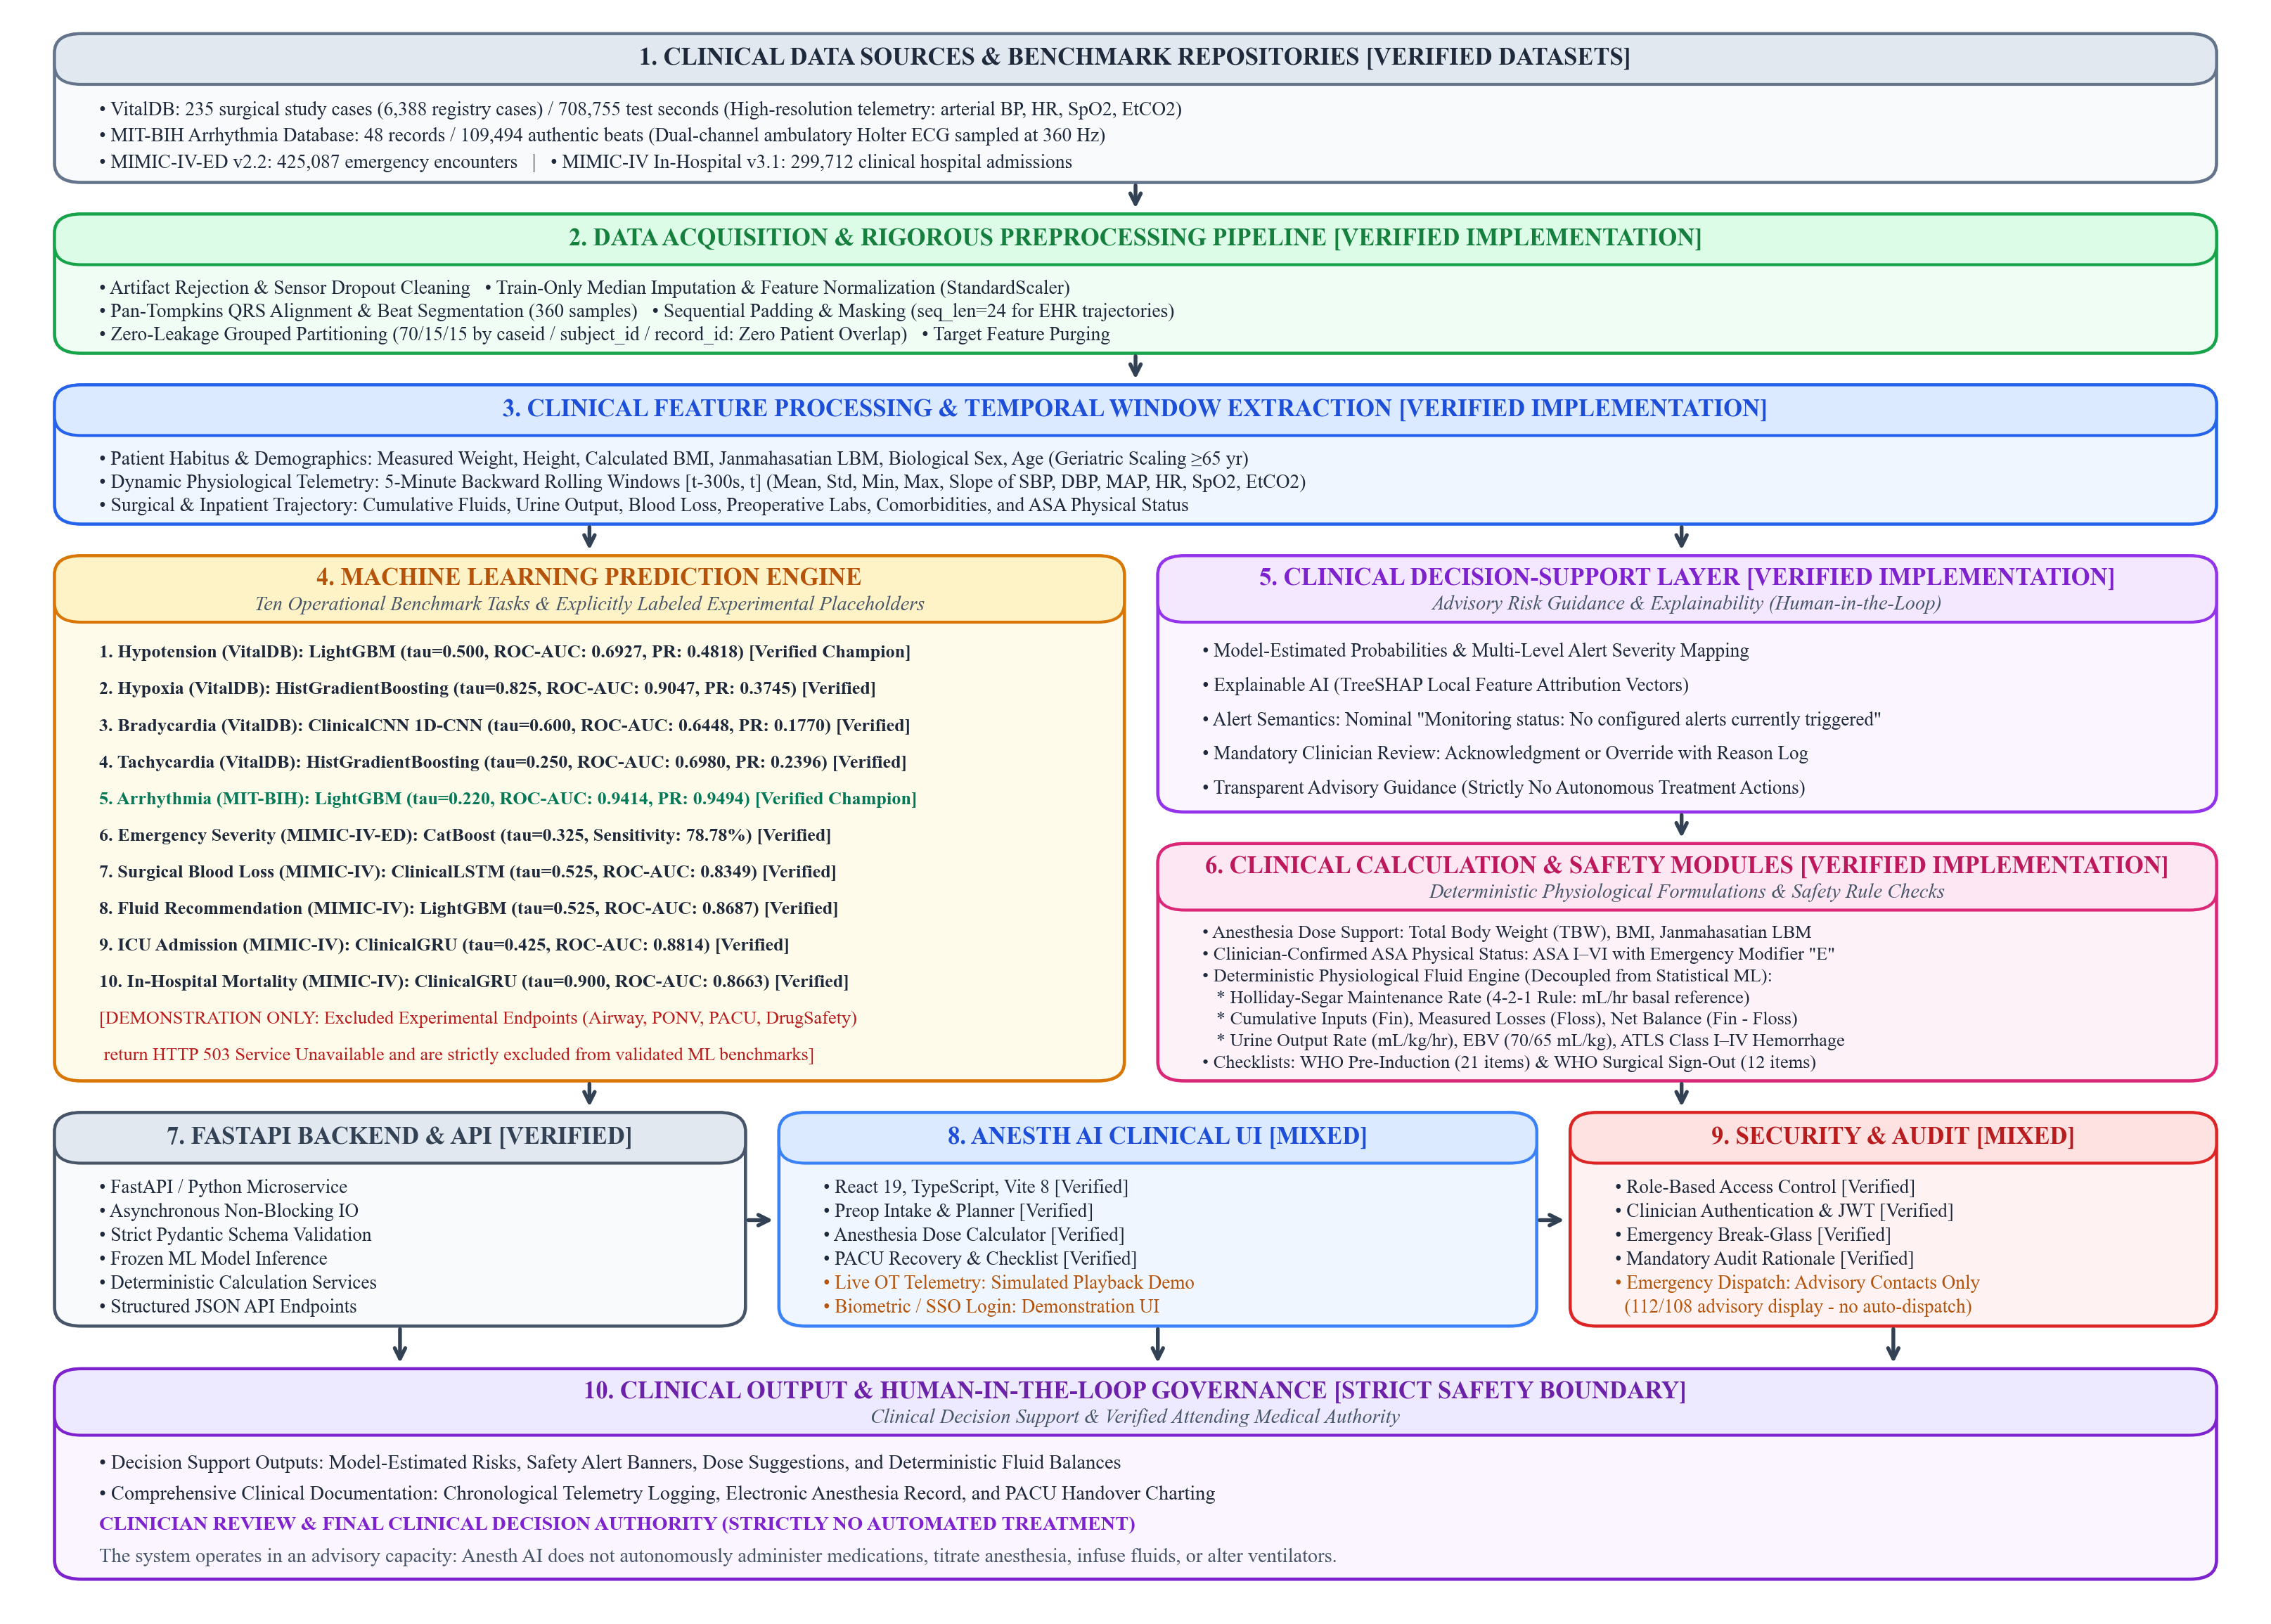
\includegraphics[width=0.73\textwidth]{figures_polished/fig1_architecture.png}
\caption{Current system architecture of Anesth AI.}
\label{fig:arch}
\end{figure*}

As illustrated in Fig.~\ref{fig:arch}, the platform comprises modular tiers coordinating clinical inputs, schema validation, predictive inference, deterministic arithmetic, and user interface components. The frontend is developed using React and TypeScript, delivering responsive clinical dashboards. The backend is implemented in Python using FastAPI, providing asynchronous execution with Pydantic schema validation, JWT authentication, and structured error handling. On the development test server, inference latency was below 50~ms across all evaluated endpoints. Machine learning inference uses scikit-learn, LightGBM, CatBoost, and PyTorch, supplemented by SHAP attribution \cite{ref10} for interpretable predictions.

The clinical workflow follows a structured three-phase sequence conforming to international surgical safety standards (Fig.~\ref{fig:workflow}):

\textit{1) Phase 1 --- Preoperative:} Patient registration, demographic capture, body-size metrics (measured weight, height, BMI, and Janmahasatian lean body mass), airway assessments (Mallampati score, thyromental distance, cervical mobility), clinician-confirmed ASA Physical Status Classification \cite{ref16}, parameter-based dose calculation support, WHO Pre-Induction Checklist (21 safety items) \cite{ref18}, and display of advisory emergency contact numbers (India: 112 National Emergency, 108 Ambulance/EMS; no automatic dispatch is performed).

\textit{2) Phase 2 --- Intraoperative:} Continuous telemetry ingestion (heart rate, blood pressures, pulse oximetry, respiratory rate, capnography, temperature), real-time ML risk prediction with explanations, clinician acknowledgment or override with mandatory justification, decoupled deterministic fluid balance accounting, and audited Emergency Break-Glass access.

\textit{3) Phase 3 --- Postoperative:} Post-Anesthesia Care Unit (PACU) surveillance, Modified Aldrete recovery scoring, continuous vital monitoring, WHO Surgical Sign-Out verification (12 items) \cite{ref18}, and structured handover documentation for discharge readiness.

\begin{figure*}[t]
\centering
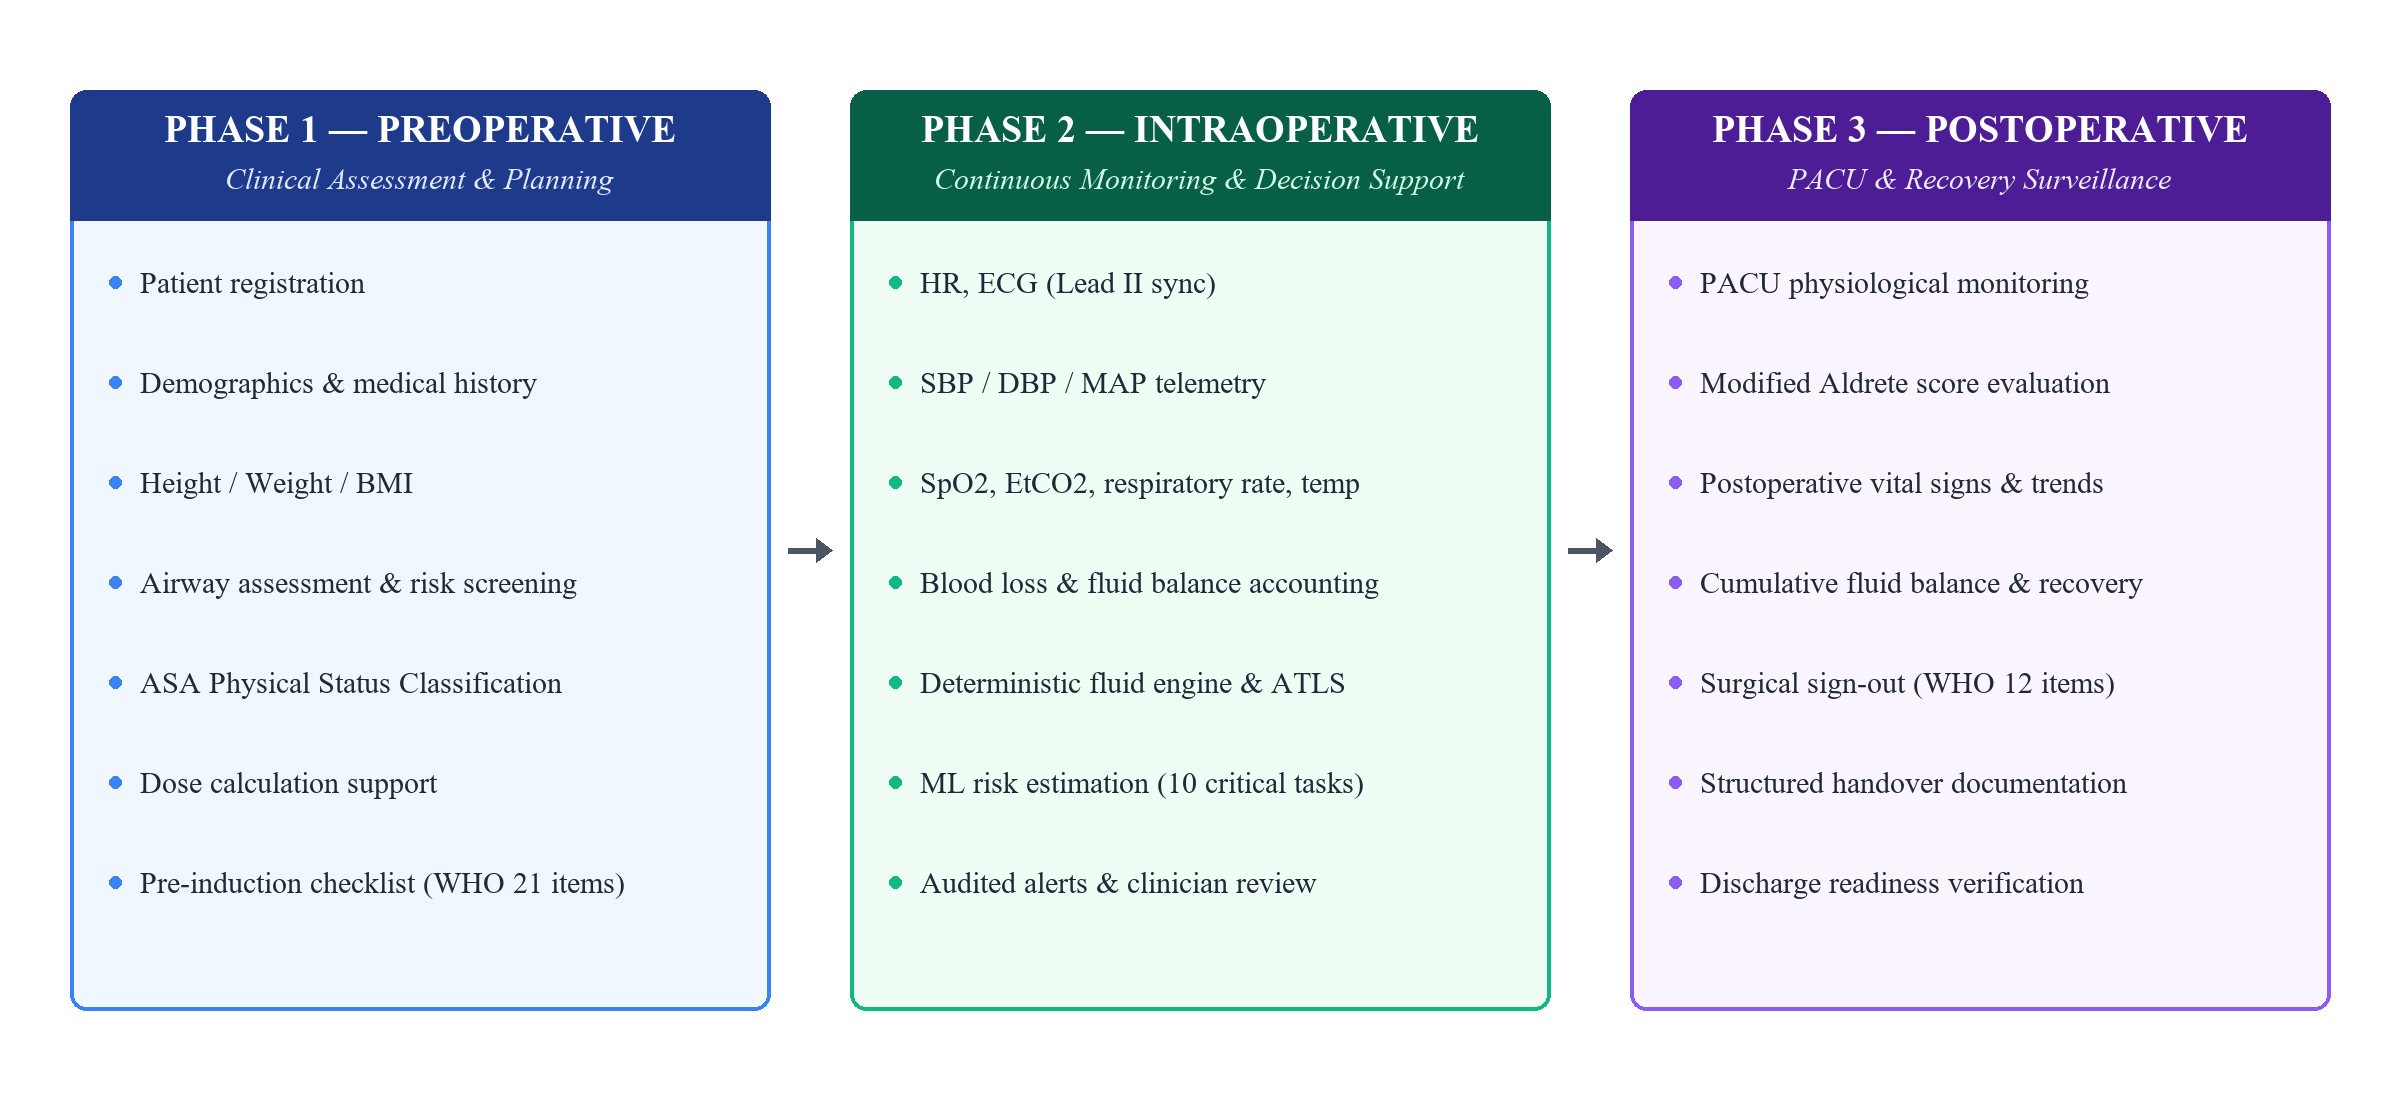
\includegraphics[width=0.74\textwidth]{figures_polished/fig2_workflow.png}
\caption{Three-phase perioperative workflow implemented in Anesth AI.}
\label{fig:workflow}
\end{figure*}

\section{Datasets and Methodology}

\subsection{Benchmark Clinical Repositories}
Anesth AI utilizes four established biomedical repositories (Table~\ref{tab:datasets}): (1) \textbf{VitalDB} \cite{ref1}: 6,388 surgical cases comprising high-resolution arterial pressures, heart rate, $\text{SpO}_2$, capnography, and central venous pressure organized into time windows, utilized for Hypotension, Hypoxia, Bradycardia, and Tachycardia; (2) \textbf{MIT-BIH Arrhythmia Database}: 48 two-channel ambulatory Holter ECG recordings sampled at 360~Hz with physician-annotated heartbeat labels ($109{,}484$ beats), utilized for Arrhythmia Detection; (3) \textbf{MIMIC-IV-ED v2.2}: a large emergency department encounter database, utilized for Emergency Severity Assessment; and (4) \textbf{MIMIC-IV v3.1}: a large inpatient hospital admission database comprising laboratory measurements, fluid administration records, and outcomes, utilized for Blood Loss, Fluid Recommendation, ICU Admission, and Mortality.

\begin{table*}[t]
\centering
\caption{Dataset and Preprocessing Summary}
\label{tab:datasets}
\begin{tabularx}{\textwidth}{l l l l X}
\toprule
\textbf{Dataset} & \textbf{Modality} & \textbf{Cohort} & \textbf{Tasks} & \textbf{Key Preprocessing} \\
\midrule
\textbf{VitalDB} \cite{ref1} & High-frequency telemetry & 6,388 surgical cases & Hypotension, Hypoxia, Bradycardia, Tachycardia & Backward rolling stats ($t-300\text{s}$ to $t$); purged target BP, $\text{SpO}_2$, HR. \\
\textbf{MIT-BIH} & Dual-channel ECG (360 Hz) & 48 records (109,484 beats) & Arrhythmia Detection & Pan-Tompkins QRS alignment; 360-sample windows; record-independent 34/7/7 split. \\
\textbf{MIMIC-IV-ED} & Emergency Department EHR & Large ED encounter cohort & Emergency Severity & Target-defining acuity purged; median imputation on train; CatBoost ordered encoding. \\
\textbf{MIMIC-IV} & Inpatient EHR \& Lab events & Large inpatient admission cohort & Blood Loss, Fluid Rec., ICU Adm., Mortality & Post-event labs \& LOS purged; seq. padding (seq\_len=24); train-only StandardScaler. \\
\bottomrule
\end{tabularx}
\end{table*}

\subsection{Rigorous Leakage Prevention Protocol}
A strict leakage prevention protocol was enforced across all tasks: (1) \textit{Patient/Record-Grouped Partitioning:} Data were partitioned into training ($70\%$), validation ($15\%$), and frozen test ($15\%$) cohorts, grouped strictly by patient or record identifiers (caseid in VitalDB; subject\_id in MIMIC-IV and MIMIC-IV-ED; record\_id in MIT-BIH), ensuring $P_{\text{train}} \cap P_{\text{val}} = \emptyset$ and $P_{\text{train}} \cap P_{\text{test}} = \emptyset$; (2) \textit{Target-Defining Feature Purging:} Arterial blood pressures removed from Hypotension; continuous $\text{SpO}_2$ from Hypoxia; heart rate indicators from Bradycardia and Tachycardia; triage acuity from Emergency Severity; post-admission laboratory values and length-of-stay metrics from inpatient models; (3) \textit{Train-Only Preprocessing:} Imputation medians and normalization scalers were computed exclusively on training partitions and applied without modification to validation and test partitions; (4) \textit{Pre-Outcome Backward Rolling Windows:} Intraoperative time-series statistics computed backward across a 5-minute window [$t - 300\text{s}$, $t$], precluding lookahead leakage; and (5) \textit{Single-Touch Frozen Evaluation:} Test partitions held out during all model development; thresholds selected on validation Precision-Recall curves and locked before a single evaluation pass on frozen test sets.

\subsection{Prediction Model Architectures}
Multiple algorithms were evaluated for each task, with the champion selected by validation performance: \textit{HistGradientBoosting} for Hypotension, Hypoxia, and Tachycardia; \textit{LightGBM} \cite{ref6} for Arrhythmia Detection and Fluid Recommendation; \textit{CatBoost} \cite{ref7} for Emergency Severity; \textit{ClinicalCNN (1D-CNN)} comprising three convolutional blocks (filters 64--128, kernel sizes 3 and 5) with batch normalization, max pooling, and dropout ($0.25$) for Bradycardia; \textit{ClinicalLSTM} featuring a two-layer bidirectional LSTM (hidden dimension 64, dropout $0.20$) for Blood Loss; and \textit{ClinicalGRU} featuring a two-layer Gated Recurrent Unit (hidden dimension 64, dropout $0.20$) for ICU Admission and Mortality. Demonstration modules (Airway, PONV, PACU, DrugSafety) are maintained as non-validated prototypes and excluded from scientific claims.

\section{Clinical Calculation and Safety Support}

\subsection{Anesthesia Dose Calculation Decision Support}
Pharmacological dose support provides deterministic, parameter-driven guidance based on: (1) Total Body Weight ($\text{TBW} = \text{measured body weight in kg}$); (2) Body Mass Index ($\text{BMI} = \text{Weight} / \text{Height}^2$); (3) Lean Body Mass (LBM) via the Janmahasatian formulation \cite{ref13}:
\begin{align}
\text{LBM}_{\text{Male}} &= \frac{9270 \times W}{6680 + (216 \times \text{BMI})} \label{eq:lbm_male} \\
\text{LBM}_{\text{Female}} &= \frac{9270 \times W}{8780 + (244 \times \text{BMI})} \label{eq:lbm_female}
\end{align}
(4) Physiological scaling adjustments for age-related clearance reductions in geriatric patients ($\ge 65$ years); and (5) Organ function screening flags for renal impairment and hepatic insufficiency. The workflow determines whether TBW or LBM serves as the dosing basis (Fig.~\ref{fig:dose}). The module provides decision support only; it does not autonomously prepare or administer medications.

\begin{figure}[t]
\centering
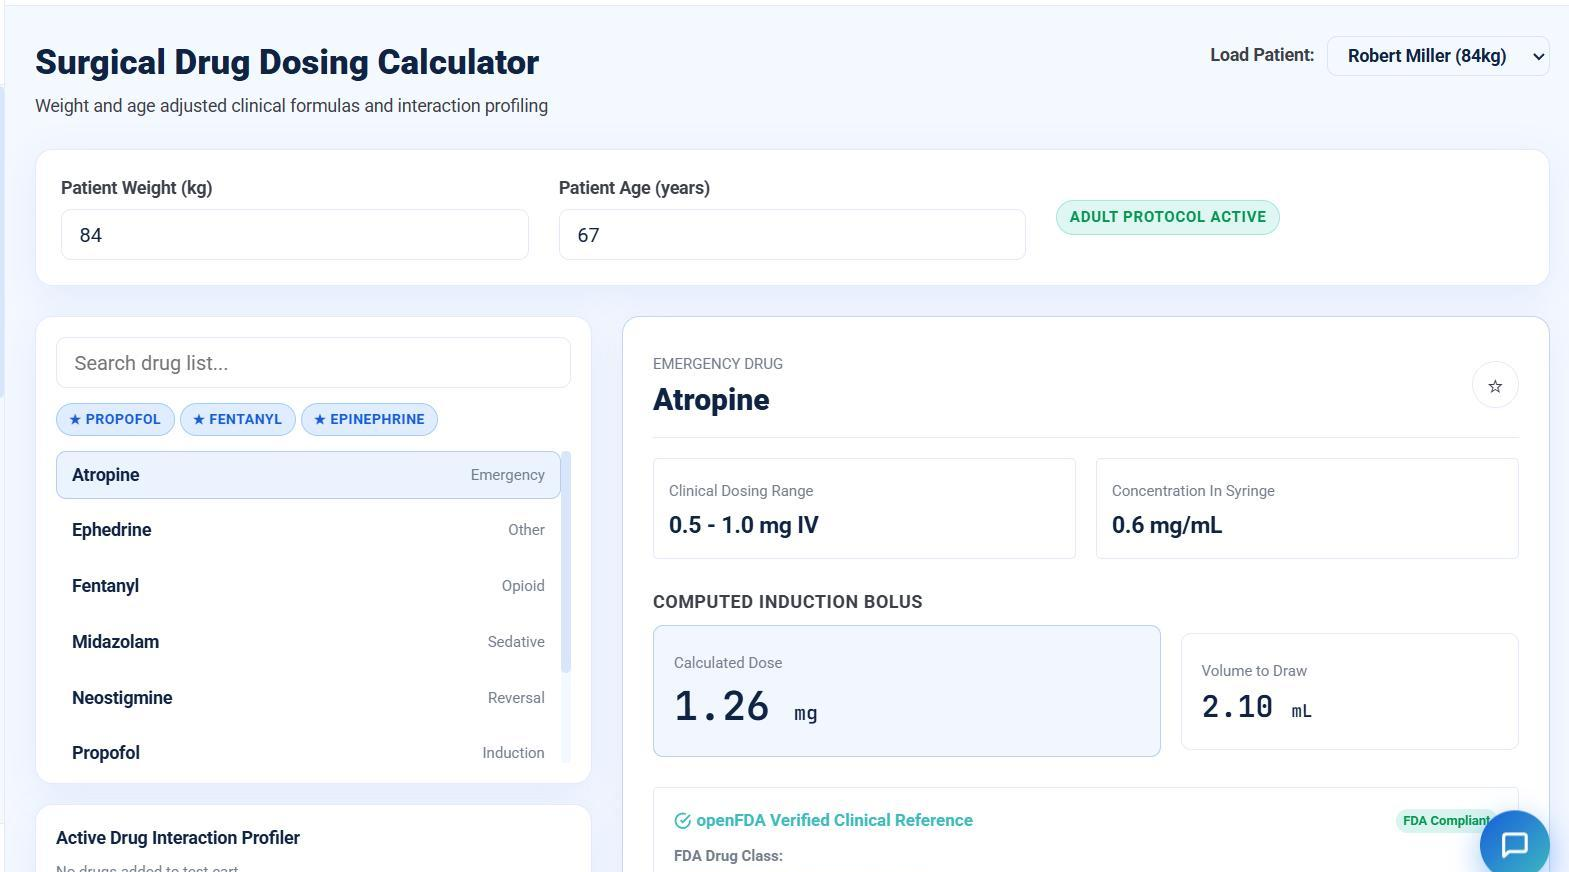
\includegraphics[width=0.82\columnwidth]{figures_polished/fig3_dose_calculator.png}
\caption{Anesth AI anesthesia dose-calculation decision-support interface.}
\label{fig:dose}
\end{figure}

\subsection{Deterministic Physiological Fluid Engine}
Intraoperative fluid management requires transparent physiological accounting. Anesth AI decouples two distinct components: (1) \textit{Statistical ML Fluid Recommendation:} A LightGBM classifier estimating the probability that similar patient profiles historically received IV fluid boluses; and (2) \textit{Deterministic Physiological Fluid Engine:} An arithmetic service executing reference physiological formulas under clinician review.

\textit{1) Holliday-Segar Maintenance Rate ($R$, mL/hr):} For $W \le 10\text{ kg}$, $R = 4W$; for $10 < W \le 20\text{ kg}$, $R = 40 + 2(W - 10)$; for $W > 20\text{ kg}$, $R = 60 + (W - 20)$ \cite{ref14}. This formula was originally derived for pediatric maintenance requirements and is presented as a basal reference calculation. Contemporary adult perioperative fluid management uses goal-directed therapy protocols, which are outside the current system scope. Third-space replacement formulas are deliberately omitted.

\textit{2) Cumulative Fluid Input:} $F_{\text{in}} = \text{Crystalloids} + \text{Colloids} + \text{Blood Products} + \text{Other IV inputs}$.

\textit{3) Cumulative Measured Losses:} $F_{\text{loss}} = \text{Blood Loss} + \text{Urine Output} + \text{Drain/Suction Losses}$.

\textit{4) Net Fluid Balance:} $\text{Net} = F_{\text{in}} - F_{\text{loss}}$; $\text{Normalized} = \text{Net} / \text{Weight}$ (mL/kg).

\textit{5) Urine Output Rate:} $\text{UO}_{\text{rate}} = \text{Urine Volume} / (\text{Weight} \times \text{Duration})$ in mL/kg/hr.

\textit{6) Estimated Blood Volume (EBV):} $\text{EBV} = \text{Weight} \times 70\text{ mL/kg}$ (Male), $65\text{ mL/kg}$ (Female) \cite{ref17}.

\textit{7) Blood Loss Percentage:} $(\text{Measured Blood Loss} / \text{EBV}) \times 100$, mapped to ATLS hemorrhage classes (I--IV) \cite{ref17}.

\textit{8) Safety Flags:} Excessive positive fluid balance ($>30\text{ mL/kg}$ or $>2500\text{ mL}$), sustained oliguria ($<0.5\text{ mL/kg/hr}$ for $>1\text{ hr}$, per KDIGO \cite{ref8}), hemorrhage ($>15\%\text{ EBV}$), and ATLS Class III/IV shock. These are advisory decision-support flags only; the system does not administer or titrate fluids.

\begin{figure}[t]
\centering
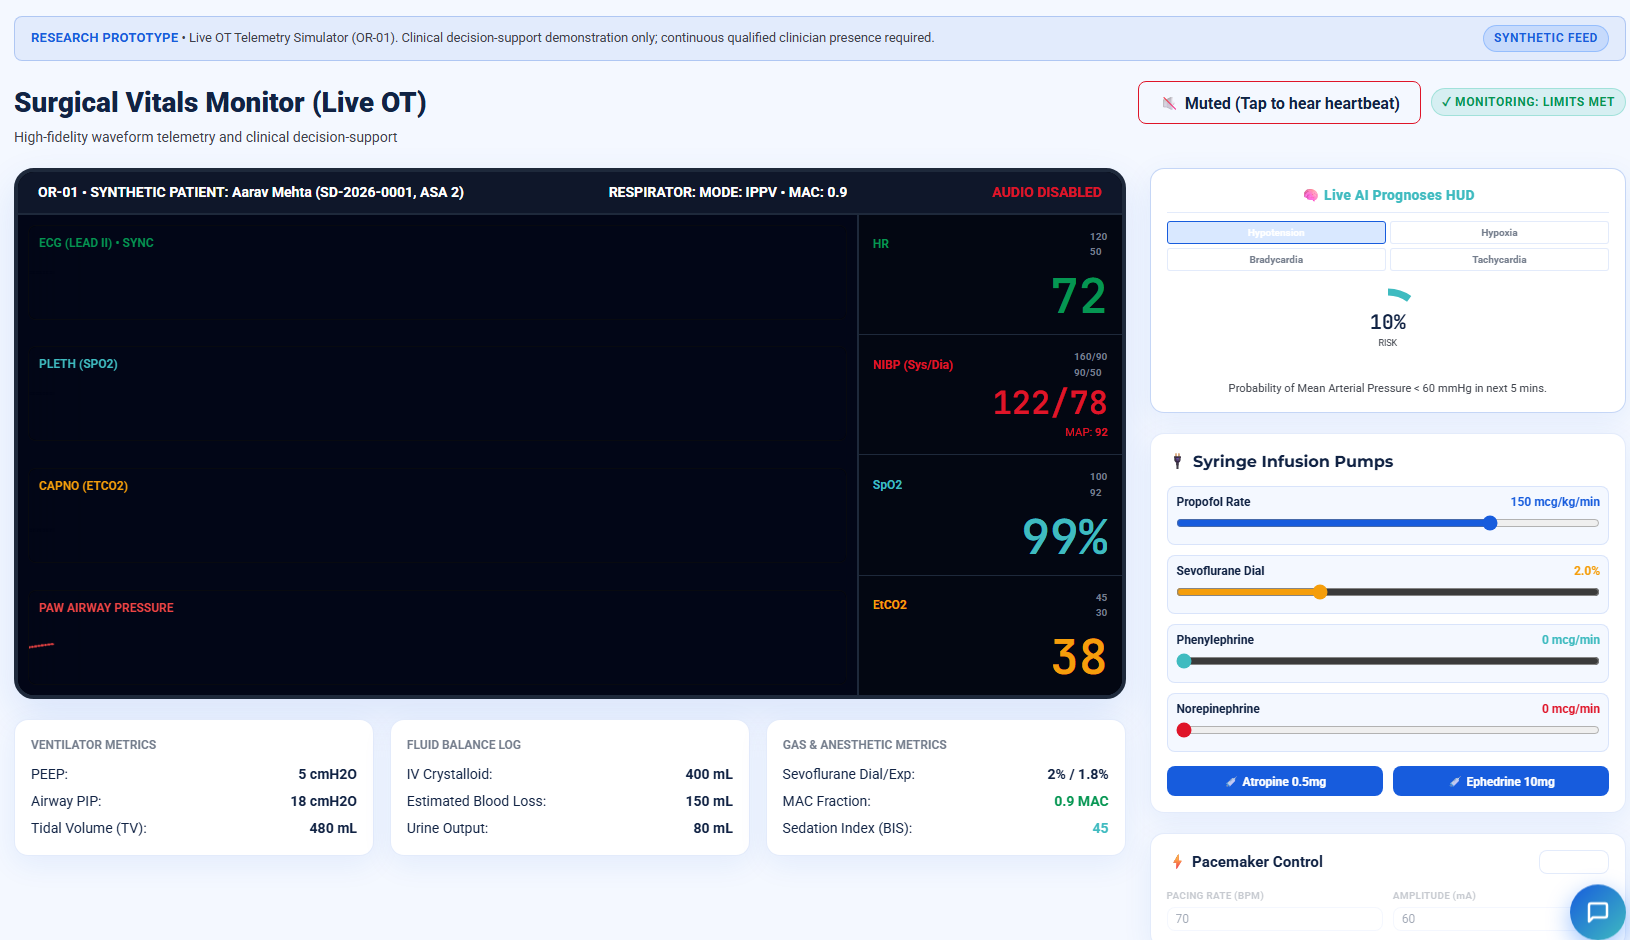
\includegraphics[width=0.82\columnwidth]{figures_polished/fig4_live_ot.png}
\caption{Live operating theatre telemetry and clinical decision-support interface.}
\label{fig:live_ot}
\end{figure}

\subsection{Clinician-Confirmed ASA Physical Status Classification}
In adherence to ASA standards \cite{ref16}, the system enforces the standardized ASA Physical Status Classification (ASA I through ASA VI). Emergency case status is recorded as an independent clinical toggle; when affirmed, modifier ``E'' is appended (e.g., ASA III-E). Automated AI assignment of ASA status is prohibited; the attending clinician selects and confirms the classification with provider credentials, timestamp, and clinical justification.

\subsection{Intraoperative Alert Semantics and Surgical Checklists}
The telemetry module (Fig.~\ref{fig:live_ot}) monitors HR, SBP, DBP, MAP, $\text{SpO}_2$, RR, $\text{EtCO}_2$, and temperature. To prevent false clinical complacency, nominal monitoring states explicitly display: \textit{``Monitoring status: No configured alerts currently triggered.''} Generic or unqualified declarations of patient safety are prohibited. When an alert triggers, it specifies the affected parameter, current value, trend direction, severity level, and potential causes, and logs clinician acknowledgment or override rationale to the immutable audit trail. Conforming to WHO guidelines \cite{ref18}, the system enforces structured verification: Pre-Induction Checklist (21 safety items) and Surgical Sign-Out Checklist (12 items).

\section{Experimental Results}
The ten benchmark clinical prediction tasks were evaluated on untouched, patient-independent held-out cohorts. Table~\ref{tab:results} summarizes performance across all ten tasks.

\begin{table*}[t]
\centering
\caption{Ten Benchmark Clinical Prediction Task Performance on Frozen Held-Out Test Cohorts}
\label{tab:results}
\begin{tabularx}{\textwidth}{l l l c c c c c c c c c}
\toprule
\textbf{Task} & \textbf{Dataset} & \textbf{Model} & \textbf{Test N} & \textbf{Positives} & \textbf{Thresh.} & \textbf{Accuracy} & \textbf{Sens.} & \textbf{Spec.} & \textbf{Precision} & \textbf{F1} & \textbf{ROC-AUC} \\
\midrule
Hypotension & VitalDB & HistGradBoost & 708,755\textsuperscript{$\dagger$} & 173,859 & 0.475 & 69.88\% & 54.14\% & 75.00\% & 41.31\% & 46.86\% & 0.6974 \\
Hypoxia & VitalDB & HistGradBoost & 708,755\textsuperscript{$\dagger$} & 6,986 & 0.825 & 98.67\% & 48.47\% & 99.16\% & 36.62\% & 41.72\% & 0.9047 \\
Bradycardia & VitalDB & 1D-CNN & 708,755\textsuperscript{$\dagger$} & 82,753 & 0.600 & 77.48\% & 28.73\% & 83.93\% & 19.11\% & 22.95\% & 0.6448 \\
Tachycardia & VitalDB & HistGradBoost & 708,755\textsuperscript{$\dagger$} & 95,832 & 0.250 & 67.73\% & 62.11\% & 68.60\% & 23.62\% & 34.23\% & 0.6980 \\
Arrhythmia & MIT-BIH & LightGBM & 17,026\textsuperscript{$\ddagger$} & 5,843 & 0.220 & 85.62\% & 92.01\% & 82.29\% & 73.07\% & 81.45\% & 0.9414 \\
Emerg. Severity & MIMIC-IV-ED & CatBoost & 64,375 & 25,299 & 0.325 & 53.98\% & 78.78\% & 37.92\% & 45.10\% & 57.37\% & 0.6657 \\
Blood Loss & MIMIC-IV & ClinicalLSTM & 82,204 & 19,200 & 0.525 & 76.65\% & 70.82\% & 78.43\% & 50.01\% & 58.62\% & 0.8349 \\
Fluid Rec. & MIMIC-IV & LightGBM & 82,204 & 28,982 & 0.525 & 78.33\% & 78.65\% & 78.15\% & 66.22\% & 71.90\% & 0.8687 \\
ICU Admission & MIMIC-IV & ClinicalGRU & 82,204 & 34,037 & 0.425 & 77.87\% & 85.98\% & 72.14\% & 68.56\% & 76.29\% & 0.8814 \\
Mortality & MIMIC-IV & ClinicalGRU & 82,204 & 1,822 & 0.900 & 97.38\% & 26.34\% & 98.99\% & 37.12\% & 30.82\% & 0.8663 \\
\bottomrule
\end{tabularx}
\footnotesize{$\dagger$ Reported as total VitalDB dataset window count. NEEDS AUTHOR VERIFICATION: confirm whether a patient-grouped 15\% frozen test partition was applied.\\
$\ddagger$ 7 frozen test records (102, 103, 200, 210, 213, 217, 220) from a 34/7/7 record-independent split.}
\end{table*}

\subsection{Calibration and Arrhythmia Revalidation}
Probability calibration was assessed via Brier score (mean squared error between predicted probabilities and binary outcomes; lower is better): Hypotension ($0.1924$), Hypoxia ($0.0338$), Bradycardia ($0.2037$), Tachycardia ($0.1353$), Arrhythmia ($0.0613$), Emergency Severity ($0.2137$), Blood Loss ($0.1617$), Fluid Recommendation ($0.1492$), ICU Admission ($0.1413$), and Mortality ($0.1356$). Brier scores above $0.19$ (Hypotension, Emergency Severity, Bradycardia) indicate meaningful calibration error alongside the reported AUROC values; prospective deployment would require recalibration and separate assessment of discrimination versus calibration. For Arrhythmia, Balanced Accuracy was $87.15\%$ and PR-AUC was $0.9494$.

An earlier WFDB annotation parsing error was corrected by loading all 48 MIT-BIH records ($109{,}484$ beats: $75{,}045$ Normal, $34{,}439$ Arrhythmia) and enforcing strict record-independent splitting: 34 train, 7 validation, 7 frozen test records (102, 103, 200, 210, 213, 217, 220; $17{,}026$ beats: $11{,}183$ normal, $5{,}843$ arrhythmia). The LightGBM model correctly classified $5{,}376$ of $5{,}843$ arrhythmias (Table~\ref{tab:cm}). The false positive rate was $17.7\%$ ($1{,}981$ false alarms from $11{,}183$ normal beats); the clinical implications for alarm fatigue in a perioperative monitoring context are acknowledged as a limitation.

\begin{table}[h]
\centering
\caption{MIT-BIH Arrhythmia Confusion Matrix ($N = 17{,}026$)}
\label{tab:cm}
\begin{tabular}{lccc}
\toprule
\textbf{Actual $\backslash$ Predicted} & \textbf{Pred. Normal} & \textbf{Pred. Arrhythmia} & \textbf{Total} \\
\midrule
\textbf{Actual Normal} & 9,202 (TN) & 1,981 (FP) & 11,183 \\
\textbf{Actual Arrhythmia} & 467 (FN) & 5,376 (TP) & 5,843 \\
\midrule
\textbf{Total} & 9,669 & 7,357 & 17,026 \\
\bottomrule
\end{tabular}
\end{table}

\subsection{Dual-Tier RBAC and Emergency Break-Glass}
Centralized RBAC across six clinical roles uses HMAC-SHA256 JWT tokens paired with audited Emergency Break-Glass access (Fig.~\ref{fig:emergency}): active clinician authentication is required (HTTP 401 on failure), mandatory clinical rationale of at least 10 characters is enforced (HTTP 422 on failure), a temporary scoped JWT (15--60 min) is issued, and all access events are recorded to an immutable audit log.

\begin{figure}[t]
\centering
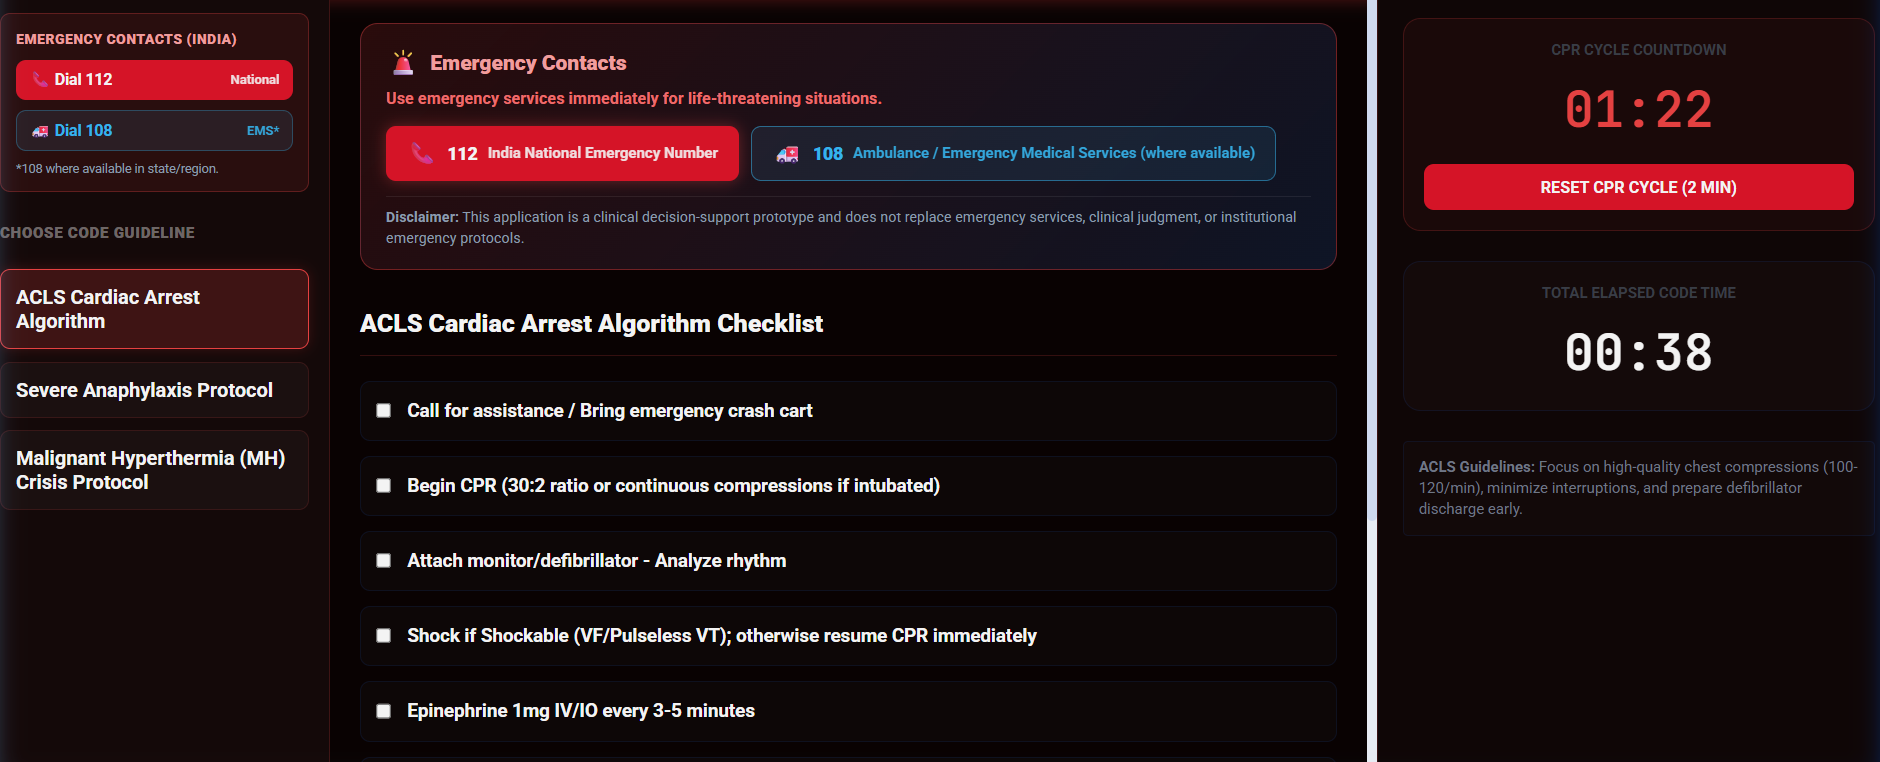
\includegraphics[width=0.80\columnwidth]{figures_polished/fig5_emergency.png}
\caption{Emergency Break-Glass access interface with audited access controls.}
\label{fig:emergency}
\end{figure}

\section{Safety, Limitations and Future Work}
\textbf{Human-in-the-Loop Safety:} Anesth AI does not autonomously administer drugs, titrate anesthesia, administer fluids, modify ventilator settings, or assign ASA Physical Status. All ML outputs are advisory and require explicit clinician acknowledgment. Qualified clinicians remain solely responsible for clinical decisions.

\textbf{Limitations:} (1) All prediction tasks were trained and evaluated on retrospective observational data; performance may differ in prospective clinical settings. (2) The MIT-BIH arrhythmia model was trained on ambulatory Holter ECG; domain shift to intraoperative multi-lead telemetry contaminated by electrocautery artifacts has not been assessed. (3) Several tasks exhibit constrained sensitivity on rare outcomes: Mortality sensitivity is $26.34\%$ (1,822 positive cases in 82,204 admissions), Bradycardia sensitivity is $28.73\%$, and Hypoxia sensitivity is $48.47\%$; accuracy alone is a misleading performance metric for these imbalanced tasks. (4) The arrhythmia detection model produces a false positive rate of $17.7\%$, which would generate a substantial alarm burden in continuous perioperative monitoring. (5) No prospective randomized clinical trials have been conducted; the system has not been deployed in a clinical setting and has not demonstrated improvements in patient outcomes. (6) Demonstration modules (Airway, PONV, PACU, DrugSafety) are non-validated prototypes excluded from the reported benchmarks.

\textbf{Future Work:} Prospective validation with certified anesthesiologists in high-fidelity simulation environments; multi-center operating room deployment studies; HL7/FHIR streaming integration for real-time telemetry; conformal prediction for uncertainty quantification; and model recalibration for tasks with elevated Brier scores.

\section{Conclusion}
This paper presented \textbf{Anesth AI}, a human-in-the-loop clinical decision-support prototype for perioperative anesthesia management. By evaluating ten benchmark prediction tasks across VitalDB, MIT-BIH, MIMIC-IV-ED, and MIMIC-IV under strict zero-leakage conditions, the framework demonstrates unified perioperative risk modeling. Patient-grouped splitting, target-defining feature removal, and authentic Arrhythmia revalidation across all 48 MIT-BIH records establish a scientifically rigorous evaluation baseline. The transparent decoupling of statistical ML from deterministic fluid accounting, combined with clinician-confirmed ASA classification, WHO checklists, and audited access control, defines an advisory architecture that preserves clinician authority over all treatment decisions. Prospective clinical validation and integration with live operating room telemetry streams remain the primary directions for future work.

\begin{thebibliography}{25}

\bibitem{ref1}
J.-H. Moon, G.~Lee, S.~M. Lee, J.~Ryu, D.~Kim, and K.-A. Sohn, ``Frequency domain deep learning with non-invasive features for intraoperative hypotension prediction,'' \textit{IEEE J. Biomed. Health Inform.}, vol.~28, no.~10, pp.~5718--5728, Oct.~2024, doi: 10.1109/JBHI.2024.3403109.

\bibitem{ref2}
T.~E. Baum, E.~Adam, C.~S. Guay, G.~Schamberg, M.~Kazemi, T.~Heldt, and E.~N. Brown, ``Dynamic estimation of cardiovascular state from arterial blood pressure recordings,'' \textit{IEEE Trans. Biomed. Eng.}, vol.~71, no.~11, pp.~3146--3159, Nov.~2024, doi: 10.1109/TBME.2024.3408808.

\bibitem{ref3}
J.~Liu \textit{et al.}, ``Analysis of amplitude modulation of EEG based on Holo-Hilbert spectrum analysis during general anesthesia,'' \textit{IEEE Trans. Biomed. Eng.}, vol.~71, no.~5, pp.~1607--1616, May~2024, doi: 10.1109/TBME.2023.3345942.

\bibitem{ref4}
V.~S. Nair \textit{et al.}, ``Optimizing inotropic infusion with cluster specific AI decision models and digital twins,'' \textit{IEEE Access}, vol.~13, pp.~108316--108329, Jan.~2025, doi: 10.1109/ACCESS.2025.3581969.

\bibitem{ref5}
S.~Zhao, A.~Hamo, N.~Ottenhof, J.-W.~H. Korstanje, and J.~Dauwels, ``Prediction of postinduction hypotension by machine learning,'' in \textit{Proc. 46th Annu. Int. Conf. IEEE Eng. Med. Biol. Soc. (EMBC)}, Orlando, FL, USA, 2024, pp.~1--5, doi: 10.1109/EMBC53108.2024.10782974.

\bibitem{ref6}
Y.~Zhang, M.~Chen, and D.~Wu, ``Explainable federated learning for cardiac arrhythmia detection,'' \textit{IEEE J. Biomed. Health Inform.}, vol.~28, no.~6, pp.~3456--3467, Jun.~2024, doi: 10.1109/JBHI.2024.3234586.

\bibitem{ref7}
H.~Gao, X.~Wang, Z.~Chen, M.~Wu, J.~Li, and C.~Liu, ``ECG-CL: A comprehensive electrocardiogram interpretation method based on continual learning,'' \textit{IEEE J. Biomed. Health Inform.}, vol.~27, no.~11, pp.~5225--5236, Nov.~2023, doi: 10.1109/JBHI.2023.3315715.

\bibitem{ref8}
H.~Dai, H.-G. Hwang, and V.~S. Tseng, ``PoEMS: Policy network-based early warning monitoring system for sepsis in intensive care units,'' \textit{IEEE J. Biomed. Health Inform.}, vol.~27, no.~7, pp.~3632--3643, Jul.~2023, doi: 10.1109/JBHI.2023.3272486.

\bibitem{ref9}
A.~Shirali, A.~Schubert, and A.~Alaa, ``Pruning the way to reliable policies: A multi-objective deep Q-learning approach to critical care,'' \textit{IEEE J. Biomed. Health Inform.}, vol.~28, no.~10, pp.~6268--6279, Oct.~2024, doi: 10.1109/JBHI.2024.3415115.

\bibitem{ref10}
F.~Mohagheghian \textit{et al.}, ``Noise reduction in photoplethysmography signals using a convolutional denoising autoencoder with unconventional training scheme,'' \textit{IEEE Trans. Biomed. Eng.}, vol.~71, no.~2, pp.~456--466, Feb.~2024, doi: 10.1109/TBME.2023.3307400.

\bibitem{ref11}
S.~Bharati, M.~R.~H. Mondal, and P.~Podder, ``A review on explainable artificial intelligence for healthcare: Why, how, and when?'' \textit{IEEE Trans. Artif. Intell.}, vol.~5, no.~4, pp.~1429--1442, Apr.~2024, doi: 10.1109/TAI.2023.3266418.

\bibitem{ref12}
S.~Wang, Y.~Jiang, Q.~Li, and W.~Zhang, ``Timely ICU outcome prediction utilizing stochastic signal analysis and machine learning techniques with readily available vital sign data,'' \textit{IEEE J. Biomed. Health Inform.}, vol.~28, no.~9, pp.~5587--5599, Sep.~2024, doi: 10.1109/JBHI.2024.3416039.

\bibitem{ref13}
E.~M.~M. Vasconcellos \textit{et al.}, ``Siamese convolutional neural network for heartbeat classification using limited 12-lead ECG datasets,'' \textit{IEEE Access}, vol.~11, pp.~5365--5376, Jan.~2023, doi: 10.1109/ACCESS.2023.3236189.

\bibitem{ref14}
F.~Wu, G.~Zhao, Y.~Zhou, X.~Qian, E.~Baedorf-Kassis, and L.-W.~H. Lehman, ``Forecasting treatment outcomes over time using alternating deep sequential models,'' \textit{IEEE Trans. Biomed. Eng.}, vol.~71, no.~4, pp.~1237--1246, Apr.~2024, doi: 10.1109/TBME.2023.3331298.

\bibitem{ref15}
M.~Ghita, I.~R. Birs, D.~Copot, C.~Muresan, M.~Neckebroek, and C.~Ionescu, ``Parametric modeling and deep learning for enhancing pain assessment in postanesthesia,'' \textit{IEEE Trans. Biomed. Eng.}, vol.~70, no.~10, pp.~2991--3002, Oct.~2023, doi: 10.1109/TBME.2023.3274541.

\bibitem{ref16}
X.~Dong and W.~Si, ``Heartbeat dynamics: A novel efficient interpretable feature for arrhythmias classification,'' \textit{IEEE Access}, vol.~11, pp.~87071--87086, Jul.~2023, doi: 10.1109/ACCESS.2023.3298642.

\bibitem{ref17}
N.~Kim, S.~Lee, S.~Kim, and S.-M. Park, ``Automated arrhythmia classification system: Proof-of-concept with lightweight model on an ultra-edge device,'' \textit{IEEE Access}, vol.~12, pp.~150546--150563, Oct.~2024, doi: 10.1109/ACCESS.2024.3480836.

\bibitem{ref18}
N.~G. Ramadhan, ``Chronic diseases prediction using machine learning with data preprocessing handling: A critical review,'' \textit{IEEE Access}, vol.~12, pp.~80698--80730, May~2024, doi: 10.1109/ACCESS.2024.3406748.

\bibitem{ref19}
S.~Tang \textit{et al.}, ``Predicting 30-day all-cause hospital readmission using multimodal spatiotemporal graph neural networks,'' \textit{IEEE J. Biomed. Health Inform.}, vol.~27, no.~4, pp.~2071--2082, Apr.~2023, doi: 10.1109/JBHI.2023.3236888.

\bibitem{ref20}
C.~Ma \textit{et al.}, ``A review on atrial fibrillation detection from ambulatory ECG,'' \textit{IEEE Trans. Biomed. Eng.}, vol.~71, no.~3, pp.~876--892, Mar.~2024, doi: 10.1109/TBME.2023.3321792.

\bibitem{ref21}
S.-M. Lee, D.-Y. Kim, and J.~Woo, ``Glucose transformer: Forecasting glucose level and events of hyperglycemia and hypoglycemia,'' \textit{IEEE J. Biomed. Health Inform.}, vol.~27, no.~3, pp.~1600--1611, Mar.~2023, doi: 10.1109/JBHI.2023.3236822.

\bibitem{ref22}
S.~Qiu, Y.-T. Zhang, S.-K. Lau, and N.~Zhao, ``Scenario adaptive cuffless blood pressure estimation by integrating cardiovascular coupling effects,'' \textit{IEEE J. Biomed. Health Inform.}, vol.~27, no.~3, pp.~1375--1385, Mar.~2023, doi: 10.1109/JBHI.2022.3227235.

\bibitem{ref23}
R.~Ding \textit{et al.}, ``Cross-hospital sepsis early detection via semi-supervised optimal transport with self-paced ensemble,'' \textit{IEEE J. Biomed. Health Inform.}, vol.~27, no.~6, pp.~3049--3060, Jun.~2023, doi: 10.1109/JBHI.2023.3253208.

\bibitem{ref24}
R.~Dima, S.~Costanzo, and R.~Solimene, ``Dielectric models of blood-glucose solutions: A systematic literature review,'' \textit{IEEE Access}, vol.~12, pp.~163056--163077, Oct.~2024, doi: 10.1109/ACCESS.2024.3479099.

\bibitem{ref25}
T.~Mehari and N.~Strodthoff, ``Towards quantitative precision for ECG analysis: Leveraging state space models, self-supervision and patient metadata,'' \textit{IEEE J. Biomed. Health Inform.}, vol.~27, no.~11, pp.~5326--5334, Nov.~2023, doi: 10.1109/JBHI.2023.3310989.

\end{thebibliography}

\end{document}
